\documentclass{beamer}
\usefonttheme[onlymath]{serif}
\usepackage[T1]{fontenc}
\usepackage[utf8]{inputenc}
\usepackage[english, icelandic]{babel}
\usepackage{amsmath}
\usepackage{amssymb}
\usepackage{amsthm}
\usepackage{gensymb}
\usepackage{parskip}
\usepackage{mathtools}
\usepackage{listings}
\usepackage{xfrac}
\usepackage{graphicx}
\usepackage{xcolor}
\usepackage{tikz}
\usetikzlibrary{calc}
\usepackage{verbatim}
\usepackage{multicol}

\DeclareMathOperator{\lcm}{lcm}
\DeclareMathOperator{\diam}{diam}
\DeclareMathOperator{\dist}{dist}
\DeclareMathOperator{\ord}{ord}
\DeclareMathOperator{\Aut}{Aut}
\DeclareMathOperator{\Inn}{Inn}
\DeclareMathOperator{\Ker}{Ker}
\DeclareMathOperator{\trace}{trace}
\DeclareMathOperator{\fix}{fix}
\DeclareMathOperator{\Log}{Log}
\newcommand\floor[1]{\left\lfloor#1\right\rfloor}
\newcommand\ceil[1]{\left\lceil#1\right\rceil}
\newcommand\abs[1]{\left|#1\right|}
\newcommand\p[1]{\left(#1\right)}
\newcommand\sqp[1]{\left[#1\right]}
\newcommand\cp[1]{\left\{#1\right\}}
\newcommand\norm[1]{\left\lVert#1\right\rVert}
\renewcommand\qedsymbol{$\blacksquare$}
\renewcommand\Im{\operatorname{Im}}
\renewcommand\Re{\operatorname{Re}}
\usepackage{color}

\definecolor{mygray}{rgb}{0.4,0.4,0.4}
\definecolor{mygreen}{rgb}{0, 0, 1}
\definecolor{myorange}{rgb}{1.0,0.4,0}

\lstset{
commentstyle=\color{mygray},
numbersep=5pt,
numberstyle=\tiny\color{mygray},
keywordstyle=\color{mygreen},
showspaces=false,
showstringspaces=false,
stringstyle=\color{myorange},
tabsize=4
}
\lstset{literate=
{æ}{{\ae}}1
{í}{{\'{i}}}1
{ó}{{\'{o}}}1
{á}{{\'{a}}}1
{é}{{\'{e}}}1
{ú}{{\'{u}}}1
{ý}{{\'{y}}}1
{ð}{{\dh}}1
{þ}{{\th}}1
{ö}{{\"o}}1
{Á}{{\'{A}}}1
{Í}{{\'{I}}}1
{Ó}{{\'{O}}}1
{Ú}{{\'{U}}}1
{Æ}{{\AE}}1
{Ö}{{\"O}}1
{Ø}{{\O}}1
{Þ}{{\TH}}1
}

\usetheme{Madrid}

\title{Gagnagrindur}
\subtitle{Listar, forgangsbiðraðir og sammengisleit}
\author{Bergur Snorrason}
\date{\today}

\graphicspath{{myndir/}}

\AtBeginSection[] {
  \begin{frame}
    \frametitle{Efnisyfirlit}
    \tableofcontents[currentsection]
  \end{frame}
}


\begin{document}

\frame{\titlepage}

\section[Listar]{Listar}

\begin{frame}
\frametitle{Listar}
\begin{itemize}

\item<1-> Listi er einföld gagnagrind notuð til að geyma gögn á skilvirkann hátt.
\item<2-> Við viljum getað:
	\begin{itemize}
		\item<3-> Bætt staki í listann.
		\item<4-> Leitað að staki í listanum.
		\item<5-> Eytt staki úr listanum.
	\end{itemize}

\end{itemize}
\end{frame}

\begin{frame}
\frametitle{Eintengdir listar}
\begin{itemize}

\item<1-> Einfaldasta (og sennilega algengasta) leiðin til að útfæra lista er með eintengdum lista (singly linked list).
\item<2-> Eintengdur listi samanstendur af nóðum.
\item<3-> Hver nóða geymir stak í listanum og upplýsingar um staðsetningu (bendi á) næstu nóðu.

\end{itemize}
\end{frame}

\begin{frame}[fragile]
	\frametitle{Útfærsla}
	\tiny
	\begin{lstlisting}[language=C++]
typedef struct snode
{
	int v;
	struct snode* n;
} node;

class llist
{
	public:
	node* h;
	node* t;
	llist()
	{
		h = NULL; t = NULL;
	}
	void add(int n)
	{
		...
	}
	bool find(int n)
	{
		...
	}
	bool del(int n)
	{
		...
	}
};
\end{lstlisting}
\end{frame}

\begin{frame}[fragile]
	\frametitle{Útfærsla}
	\tiny
	\begin{lstlisting}[language=C++]
void add(int n)
{
	node* a = new node;
	a->v = n;
	a->n = NULL;
	if (h == NULL)
	{
		h = a; t = a;
	}
	else
	{
		t->n = a;
		t = t->n;
	}
}
\end{lstlisting}
\end{frame}

\begin{frame}[fragile]
	\frametitle{Útfærsla}
	\tiny
	\begin{lstlisting}[language=C++]
bool find(int n)
{
	node* g = h;
	while (g != NULL)
	{
		if (g->v == n)
		{
			break;
		}
		g = g->n;
	}
	return g != NULL;
}
\end{lstlisting}
\end{frame}

\begin{frame}[fragile]
	\frametitle{Útfærsla}
	\tiny
	\begin{lstlisting}[language=C++]
bool del(int n)
{
	if (h->v == n)
	{
		if (h == t)
		{
			delete h; h = NULL; t = NULL; return true;
		}
		node* g = h; h = h->n; delete g; return true;
	}
	node* gg = h; node* g = h->n;
	while (g != NULL)
	{
		if (g->v == n)
		{
			break;
		}
		gg = g; g = g->n;
	}
	if (g == NULL)
	{
		return false;
	}
	gg->n = g->n;
	if (g == t)
	{
		t = gg;
	}
	delete g;
	return true;
}
\end{lstlisting}
\end{frame}

\begin{frame}
\frametitle{Kostir og gallar}
\begin{itemize}

\item<1-> Gallar:
	\begin{itemize}
		\item<2-> Mjög hæg leit.
		\item<3-> Býður ekki upp á handahófskennda vísun (e. random access).
	\end{itemize}
\item<4-> Kostir:
	\begin{itemize}
		\item<5-> Er hluti af \texttt{C++ STL}.
		\item<6-> Unnt er að skeyta saman listum í $\mathcal{O}(1)$, eitthvað sem er
			til dæmis ekki unnt með \texttt{vector} í \texttt{C++}.
	\end{itemize}

\end{itemize}
\end{frame}

\begin{frame}
\frametitle{Tímaflækjur}
\begin{itemize}

\item<1-> Innsetning: $\mathcal{O}(1)$.
\item<2-> Leita að staki: $\mathcal{O}(n)$.
\item<3-> Eyða taki: $\mathcal{O}(n)$.

\end{itemize}
\end{frame}

\section[Forgangsbiðraðir]{Forgangsbiðraðir}

\begin{frame}
\frametitle{Forgangsbiðraðir}
\begin{itemize}

\item<1-> Forgangsbiðraðir (e. priority queues) eru þægilegar gagnagrindur að hafa.
\item<2-> Við notum þær til að geyma röðuð gögn.
\item<3-> Við viljum getað:
	\begin{itemize}
		\item<4-> Bætt staki í biðröðina.
		\item<5-> Fundið \emph{besta} stakið í biðröðinni.
		\item<6-> Eytt besta stakinu úr biðröðinni.
	\end{itemize}

\end{itemize}
\end{frame}

\begin{frame}
\frametitle{Hrúgur}
\begin{itemize}

\item<1-> Algengasta leiðin til að útfæra forgangsbiðraðir er að nota hrúgu (e. heap)
\item<2-> Hrúga er tvíundartré sem uppfyllir \emph{hrúguskilyrðinu}.
\item<3-> \emph{Hrúguskilyrðið}: Sérhver nóða er betri en, eða jafn góð, börnum sínum.

\end{itemize}
\end{frame}

\begin{frame}
\frametitle{Framsetning hrúga í tölvum}
\begin{itemize}

\item<1-> Hrúgur eru nokkuð einfaldar í útfærslu.
\item<2-> Hægt er að tákna \emph{tréð} sem \emph{fylki}.
\item<3-> Helsta atriðið verður að útfæra \emph{hrúguskilyrðis lagara}.
\item<4-> Þegar tvíundartré eru útfærð með fylkjum er yfirleitt notuð önnur af tveimur aðferðum.

\end{itemize}
\end{frame}

\begin{frame}
\frametitle{Fylki sem tré}
\begin{itemize}

\item<1-> Sú fyrri:
	\begin{itemize}
		\item<2-> Rótin er í staki $1$ í fylkinu.
		\item<3-> Vinstra barn staksins $i$ er stak $2\times i$.
		\item<4-> Hægra barn staksins $i$ er stak $2\times i + 1$.
		\item<5-> Foreldri staks $i$ er stakið $\left \lfloor \dfrac{i}{2} \right \rfloor$.
	\end{itemize}
\item<6-> Sú seinni:
	\begin{itemize}
		\item<7-> Rótin er í staki $0$ í fylkinu.
		\item<8-> Vinstra barn staksins $i$ er stak $2\times i + 1$.
		\item<9-> Hægra barn staksins $i$ er stak $2\times i + 2$.
		\item<10-> Foreldri staks $i$ er stakið $\left \lfloor \dfrac{i - 1}{2} \right \rfloor$.
	\end{itemize}

\end{itemize}
\end{frame}

\begin{frame}[fragile]
	\frametitle{Hrúgur í \texttt{C}}
	\tiny
	\begin{lstlisting}[language=C]
#define PARENT(i) ((i - 1)/2)
#define LEFT(i)   ((i)*2 + 1)
#define RIGHT(i)  ((i)*2 + 2)
int h[1000000];
int hn = 0;

void fix_down(int i)
{
	...
}

void fix_up(int i)
{
	...
}

void pop()
{
	...
}

int peek()
{
	...
}

void push(int x)
{
	...
}
\end{lstlisting}
\end{frame}

\begin{frame}[fragile]
	\frametitle{Hrúgur í \texttt{C}}
	\tiny
	\begin{lstlisting}[language=C]
void pop()
{
	hn--;
	h[0] = h[hn];
	fix_down(0);
}

int peek()
{
	return h[0];
}

void push(int x)
{
	h[hn++] = x;
	fix_up(hn - 1);
}
\end{lstlisting}
\end{frame}

\begin{frame}[fragile]
	\frametitle{Hrúgur í \texttt{C}}
	\tiny
	\begin{lstlisting}[language=C]
void fix_down(int i)
{
	int mx = i;
	if (RIGHT(i) < hn && h[mx] < h[RIGHT(i)])
	{
		mx = RIGHT(i);
	}
	if (LEFT(i) < hn && h[mx] < h[LEFT(i)])
	{
		mx = LEFT(i);
	}
	if (mx != i)
	{
		int s = h[i];
		h[i] = h[mx];
		h[mx] = s;
		fix_down(mx);
	}
}
\end{lstlisting}
\end{frame}

\begin{frame}[fragile]
	\frametitle{Hrúgur í \texttt{C}}
	\tiny
	\begin{lstlisting}[language=C]
void fix_up(int i)
{
	if (i == 0)
	{
		return;
	}
	else if (h[i] > h[PARENT(i)])
	{
		int s = h[i];
		h[i] = h[PARENT(i)];
		h[PARENT(i)] = s;
		fix_up(PARENT(i));
	}
}
\end{lstlisting}
\end{frame}

\begin{frame}
\frametitle{Kostir og gallar}
\begin{itemize}

\item<1-> Gallar:
	\begin{itemize}
		\item<2-> Styður ekki beint almenna leit.
		\item<3-> Styður ekki beint samruna.
	\end{itemize}
\item<4-> Kostir:
	\begin{itemize}
		\item<5-> Er hluti af \texttt{C++ STL}.
		\item<6-> Heldur kvikt utan um röðun.
	\end{itemize}

\end{itemize}
\end{frame}

\begin{frame}
\frametitle{Tímaflækjur}
\begin{itemize}

\item<1-> Finna \emph{besta} stakið: $\mathcal{O}(1)$.
\item<2-> Innsetning: $\mathcal{O}(\log n)$.
\item<3-> Eyða \emph{besta} stakinu: $\mathcal{O}(\log n)$.

\end{itemize}
\end{frame}



\section[Sammengisleit]{Sammengisleit}

\begin{frame}
\frametitle{Sammengisleit}
\begin{itemize}

\item<1-> Sammengisleit (e. union-find) er öflug leið til að halda utan um jafngildisflokka tiltekna vensla,
	eða m.ö.o. halda utan um \emph{sundurlæg} mengi.
\item<2-> Við viljum getað:
	\begin{itemize}
		\item<3-> Borið saman samhengisþætti mismunandi staka.
		\item<4-> Sameinað samhengisflokka.
	\end{itemize}
\item<5-> Við tölum um aðgerðirnar \texttt{find(x)} og \texttt{join(x, y)}.

\end{itemize}
\end{frame}

\begin{frame}
\frametitle{Dæmi}
\begin{itemize}

	\item<1-> Tökum sem dæmi einstökungasafnið
		$\{\{1\}, \{2\}, \{3\}, \{4\}, \{5\}\}$. 
	\item<2-> \texttt{join(1, 3)} gefur okkur
		$\{\{1, 3\}, \{2\}, \{4\}, \{5\}\}$. 
	\item<3-> \texttt{join(2, 5)} gefur okkur
		$\{\{1, 3\}, \{2, 5\}, \{4\}\}$. 
	\item<4-> \texttt{join(2, 4)} gefur okkur
		$\{\{1, 3\}, \{2, 4, 5\}\}$. 
	\item<5-> \texttt{join(1, 4)} gefur okkur
		$\{\{1, 2, 3, 4, 5\}\}$. 
	\item<6-> Á sérhverjum tímapunkti myndi \texttt{find(x)} skila einhverju staki sem er í sama mengi og \texttt{x}.
	\item<7-> Aðalatriðið er að \texttt{find(x)} skilar sama stakinu fyrir sérhvert stak í sérhverjum samhengisflokki.
	\item<8-> Til dæmis, í þriðja punktinum myndi \texttt{find(1)} og \texttt{find(3)} alltaf skila sama stakinu.
\end{itemize}
\end{frame}

\begin{frame}
\frametitle{Útfærsla á frumstæðri sammengisleit}
\begin{itemize}
	\item<1-> Gerum ráð fyrir að tölurnar sem við munum vinna með séu jákvæðar og minni en $n$.
	\item<2-> Við munum þá gefa okkur $n$ staka fylki $p$, þar sem $i$-ta stakið í fylkinu er upphafstillt sem $i$.
	\item<3-> Fylkið $p$ mun nú geyma \emph{foreldri} sérhvers stak.
	\item<3-> Foreldrin myndi keðjur.
	\item<4-> Sérhver keðja endar í einhverju staki, sem við munum kalla \emph{ráðherra} jafngildisflokksins.
\end{itemize}
\end{frame}

\begin{frame}
\frametitle{Mynd af keðjum}
	Keðjurnar sem fást með $\{\{0, 2, 4, 5, 9, 10\}, \{1, 3, 6, 11\}, \{7, 8\}\}$ gætu til dæmis verið
	gefnar með $p = [0, 1, 0, 1, 0, 4, 3, 7, 7, 5, 5, 3]$.
	\begin{figure}
	\item<2->
		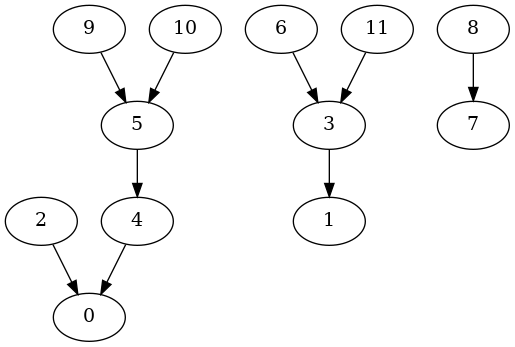
\includegraphics[scale=0.5]{mynd.png}
	\end{figure}
\end{frame}

\begin{frame}
\frametitle{Útfærsla á frumstæðri sammengisleit}
\begin{itemize}
	\item<1-> Til að fá ráðherra flokks tiltekins staks er hægt að fara endurkvæmt upp keðjuna.
	\item<2-> Til að sameina flokka nægir að breyta foreldri ráðherra annars flokksins yfir í
		eitthvert stak hins flokksins (sér í lagi ráðherra þess).
	\item<3-> Báðar þessar aðgerðir er auðvelt að útfæra.
\end{itemize}
\end{frame}

\begin{frame}[fragile]
	\frametitle{Frumstæð sammengisleit}
\tiny
\begin{lstlisting}[language=C++]
int p[MAX];

int find(int x)
{
	if (p[x] == x)
	{
		return x;
	}
	else
	{
		return find(p[x]);
	}
}

void join(int x, int y)
{
	p[find(x)] = find(y);
}

int main()
{
	int i;
	int n = MAX;
	for (i = 0; i < n; i++)
	{
		p[i] = i;
	}
	...
}
\end{lstlisting}
\end{frame}

\begin{frame}
\frametitle{Tímaflækjur frumstæðri sammengisleitar}
\begin{itemize}
	\item<1-> Við sjáum nú að tímaflækja \texttt{find} er línuleg í lengd keðjunnar, svo 
		þar sem lengd keðjunnar getur verið, í versta falli, $n$ þá er \texttt{find} $\mathcal{O}(n)$.
	\item<2-> Fallið \texttt{join} gerir lítið annað en að kalla tvisvar á \texttt{find} svo það er líka
		$\mathcal{O}(n)$.
	\item<3-> Er samt ekki hægt að bæta þetta eitthvað?
	\item<4-> Það er vissulega hægt!
\end{itemize}
\end{frame}

\begin{frame}
\frametitle{Keðjuþjöppuð sammengisleit}
\begin{itemize}
	\item<1-> Eins og nafnið á glæruni gefur til kynna er hugmyndin að þjappa keðjunum saman í hvert skipti sem kallað er á
		\texttt{find}.
	\item<2-> Þetta er gert með því að setja \texttt{p[x]} sem ráðherra flokks \texttt{x}, í hverju skrefi endurkvæmninnar.
\end{itemize}
\end{frame}

\begin{frame}
\frametitle{Dæmi um keðjuþjöppun}
\begin{itemize}
	\item<1-> Gefum okkur
		$p = [0, 0, 1, 2, 3, 4, 5, 6, 7]$.
	\item<2-> Ljóst er að \texttt{find(5)} skilar $0$.
	\item<3-> Ef við notum frumstæða sammengisleit breytist $p$ ekki neitt þegar kallað er á \texttt{find}
		en með keðjuþjappaðri sammengisleit þjappast keðjan frá og með $5$ og því fæst
		$p = [0, 0, 0, 0, 0, 0, 5, 6, 7]$.
\end{itemize}
\end{frame}

\begin{frame}[fragile]
	\frametitle{Keðjuþjöppað sammengisleit}
\tiny
\begin{lstlisting}[language=C++]
int p[MAX];

int find(int x)
{
	if (p[x] == x)
	{
		return x;
	}
	else
	{
		p[x] = find(p[x]);	//keðjuþjöppunin á sér stað í þessar línu
		return p[x];
	}
}

void join(int x, int y)
{
	p[find(x)] = find(y);
}

int main()
{
	int i;
	int n = MAX;
	for (i = 0; i < n; i++)
	{
		p[i] = i;
	}
	...
}
\end{lstlisting}
\end{frame}

\begin{frame}
\frametitle{Tímaflækjur keðjuþjappaðar sammengisleitar}
\begin{itemize}
	\item<1-> Það er flóknara að lýsa tímaflækju keðjuþjappaðrar sammengisleitar.
	\item<2-> \emph{Á heildina litið} (e. amortized) er tímaflækjan er $\mathcal{O}(\alpha(n))$, þar sem $\alpha$ er andhverfa \emph{Ackermann} fallsins.
	\item<3-> Fyrir þau $n$ sem við fáumst við er $\alpha(n)$ nánast fast.
\end{itemize}
\end{frame}

\section[Forskot á sæluna]{Forskot á sæluna}

\begin{frame}[fragile]
\frametitle{Forskot á sæluna}
\begin{itemize}

\item<1-> Forgangsbiðraðir eru notaðar í reiknirit Dijkstra.
\item<2-> Sammengisleit er notuð í reiknirit Kruskals.
\item<3-> Við munum nota hrúgur aftur í næstu viku.

\end{itemize}
\end{frame}

\end{document}
